\chapter{Total Internal Reflection}\label{lec:lec32}

In this chapter, we will discuss a special case of reflection in a dielectric boundary called Total Internal Reflection. We studied total internal reflection at the high school level where we said the ray is incident at an angle greater than the critical angle and the power is reflected in the same medium. However, that understanding is a rather superficial one. Here we do a detailed study of the phenomenon called TOTAL INTERNAL REFLECTION.

\section{Snell's Law}
From Snell's Law,
\begin{align}
\beta_1 \sin\theta_i = \beta_2 \sin\theta_t
\end{align}
where $\beta_1 and \beta_2$ are the phase constants in the two media. Writing eqn(32.1) in terms of medium parameters
\begin{align*}
\omega\sqrt{\mu_1\epsilon} \sin\theta_i = \omega\sqrt{\mu_2\epsilon_2}  \sin\theta_t
\end{align*}
\begin{center}
or
\end{center}
\begin{align*}
\sqrt{\mu_1\epsilon} \sin\theta_i = \sqrt{\mu_2\epsilon_2}  \sin\theta_t
\end{align*}
If medium parameters become such that
\begin{align}
\frac{\beta_1}{\beta_2}\sin\theta_i > 1
\end{align}then there is no wave nature in medium 2 for which the angle $\sin\theta_t$ is propagating. It's more of an imaginary angle which lacks direction.
And even though phase conditions in eq(32.1) is satisfied, there is no physical angle $\theta_t$ for which
\begin{align}
\sin\theta_t > 1
\end{align}
This poses a very interesting case. Now we require in our reflection co-efficient expression that the quantity
\begin{align}
\cos\theta_t = \sqrt{1-\sin^2\theta_t}
\end{align}
\begin{center}
Substituting eq.(32.2) in eq.(32.4)
\end{center}
\begin{align*}
\cos\theta_t = \sqrt{1-(\frac{\beta_1}{\beta_2}\sin\theta_i)^2}
\end{align*}
this leaves the quantity $-(\frac{\beta_1}{\beta_2}\sin\theta_i)^2$ always negative and imaginary.So we make it positive to satisfy the medium parameter in which $\frac{\beta_1}{\beta_2}\sin\theta_i > 1$
\begin{align}
\cos\theta_t = \jmath\sqrt{(\frac{\beta_1}{\beta_2}\sin\theta_i)^2-1}
\end{align}
Now again, we see that from Eqn (32.3) and Eqn (32.5) 
that there is no physical angle $\theta_t$ in which the wave would be propagated.

However for the angle $\theta_t$ and $\theta_i$ we would still have reflection and transmission coefficients, so we go back and substitute $\cos\theta_t$ in the reflection co-efficient expression.

Recall we had two cases of reflection coefficients.
\begin{align*}
\end{align*}For the Perpendicular case:
\begin{equation}
\Gamma_\perp\ = \frac{\eta_2\cos\theta_i - \eta_1\cos\theta_t}{\eta_2\cos\theta_i + \eta_1\cos\theta_t}
\end{equation}

For the Parallel case:
\begin{equation}
\Gamma_\parallel = \frac{\eta_1\cos\theta_i - \eta_2\cos\theta_t}{\eta_1\cos\theta_i + \eta_2\cos\theta_t}
\end{equation}
Note: $\eta_1$ and $\eta_2$ are interchanged for both cases otherwise they are similar. 

substituting eqn(32.5) in eqn(32.7)
\begin{align}
\Gamma_\parallel = \frac{\eta_1\cos\theta_i - \jmath\eta_2\sqrt{(\frac{\beta_1}{\beta_2}\sin\theta_i)^2-1}}{\eta_1\cos\theta_i + \jmath\eta_2\sqrt{(\frac{\beta_1}{\beta_2}\sin\theta_i)^2-1}}
\end{align}
Note: we would get the same expression for the perpendicular polarization case but with $\eta_1$ and $\eta_2$ interchanged. 

What's important to note here is that the expression in Eqn (32.8) is of the form
\begin{equation}
\frac{a - \jmath b}{b + \jmath b}
\end{equation}
and always have a magnitude equal  to 1 and an angle $\angle-\tan^-1(\frac{b}{a})$ that is:
\begin{equation}
|\frac{a - \jmath b}{a + \jmath b}| = 1\angle - 2\tan^{-1}(\frac{b}{a})
\end{equation} 
And since the modulus of the reflection coefficient is 1, whatever the incidence or the media is totally reflected.

\section{Conditions For Total Internal Reflection}
\begin{enumerate}[(i)]
\item If total internal reflection has to take place then,
\begin{equation*}
\frac{\beta_1}{\beta_2}\sin\theta_i > 1
\end{equation*}
in terms of medium parameters
\begin{equation*}
\frac{\sqrt{\mu_1\epsilon_1}}{\sqrt{\mu_2\epsilon_2}}\sin\theta_i > 1
\end{equation*}
$\theta_i$ can attain a maximum value of $90^\bullet$, therefore $\sin\theta_i$ = $\sin$90 = 1, this means,
\begin{equation}
\sqrt{\mu_1\epsilon_1} > \sqrt{\mu_2\epsilon_2}
\end{equation}
and there is a possibility of total internal reflection.

For non-magnetic material, $\mu_1$ and $\mu_2$
\begin{equation*}
\sqrt{\epsilon_1} > \sqrt{\epsilon_2}
\end{equation*}
\begin{align*}
n_1 > n_2
\end{align*} \begin{center}
$n_1$ and $n_2$ are refractive indexes
\end{center} 
Now the angle at which $\sin\theta_t = 1$ is called the CRITICAL ANGLE, beyond which if an incident wave is launched, there would be no transmitted wave in the second medium.

Explaining this phenomenon with fig 32.1 below.
\begin{figure}[h]
\centering
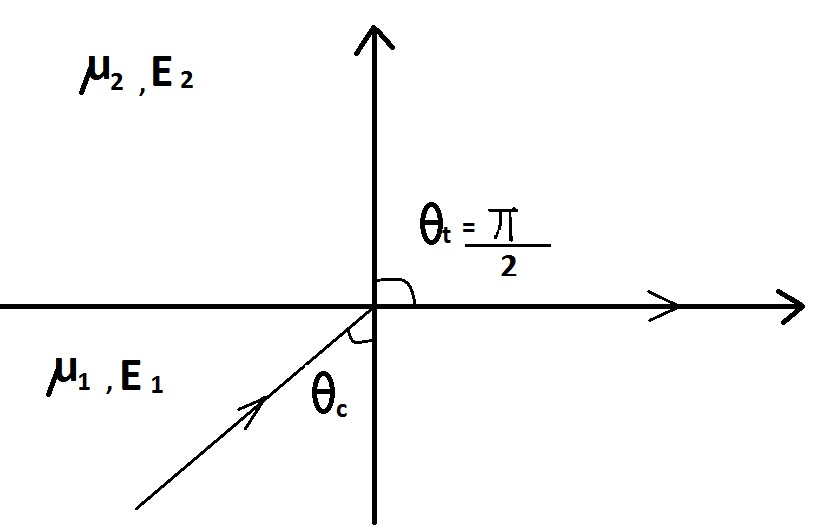
\includegraphics[width=.7\linewidth]{\pathtopartone/graphics/fig321}
\caption{graph of critical angle}
\end{figure}

\begin{equation*}
\sqrt{\mu_1\epsilon_1} \sin\theta_c = \sqrt{\mu_2\epsilon_2}
\end{equation*}
\begin{align*}
n_1 \sin\theta_c = n_2
\end{align*}
Or the critical angle
\begin{align*}
\theta_c = \sin^{-1}(\frac{n_2}{n_1}) 
\end{align*}
So in general, we can say that by choosing appropriate parameters for the media, and the angle of incidence, we can generate an arbitrary phase difference between the incidence and the reflected ray. This would happen for both parallel and perpendicular polarization. However, the parallel and perpendicular polarization have $\eta_1$ and $\eta_2$
interchanged between them. So a and b in $\frac{a - \jmath b}{b + \jmath b}$ are different for parallel and perpendicular polarizations. This means that the phase change which the wave undergoes for the two polarization is different.

\item Wave undergoes a phase change at Total Internal Reflection

The phase change is different for parallel and perpendicular polarizations.

If we write out explicitly:
\begin{equation}
\phi_\parallel = -2\tan^{-1}\frac{\eta_2\sqrt{(\frac{\beta_1}{\beta_2}\sin\theta_i)^2-1}}{\eta_1\cos\theta_i}
\end{equation}
\begin{equation}
\phi_\perp = -2\tan^{-1}\frac{\eta_1\sqrt{(\frac{\beta_1}{\beta_2}\sin\theta_i)^2-1}}{\eta_2\cos\theta_i}
\end{equation}
From here we see that the two polarization do not undergo a phase change. But later we'll see the implication of the phase change for the different kinds of polarization when Total Internal Reflection takes place in the dielectric boundary. 

\item For fields in medium 2

Recall:

The phase expression for a transmitted wave in medium 2 is
\begin{equation*}
\varepsilon_t = e^{-\jmath \beta_2(x\sin\theta_t + z\cos\theta_t)}
\end{equation*}
From Snell's Law and keeping phase gradient same $\varepsilon_t$ is written out explicitly as:
\begin{align}
\varepsilon_te^{- \jmath x\beta_2\sin\theta_t - \jmath z\beta_2\cos\theta_t}
\end{align}
substituting for $\cos\theta_t$ from Eqn (32.5)
and $\sin\theta_t$ from Eqn (32.1)
\begin{equation}
\varepsilon_te^{- {\jmath x\beta_1\sin\theta_i} - z \beta_2\sqrt{{(\frac{\beta_1}{\beta_2}\sin\theta_i)}^2 - 1}}
\end{equation}
From the above equation,

Amplitude term:
\begin{equation}
-z\sqrt{\beta_1^2\sin^2\theta_i - \beta_2}
\end{equation}
\begin{align*}
\end{align*}
and the phase term:
\begin{equation}
e^{- \jmath x\beta_1\sin\theta_i}
\end{equation}
From these equations, we see the field is exponentially dying down as a function of z and a phase which varies as a function of x.
\end{enumerate}
Now with total internal reflection, the travelling wave nature is only in the z-direction. The fields are no longer travelling in x direction.

Explicitly, eqn(32.16) essentially represents decaying fields and Eqn (32.17) gives a travelling wave in x direction. The graph of this field is shown in the plot fig 32.2
\begin{figure}[h]
\centering
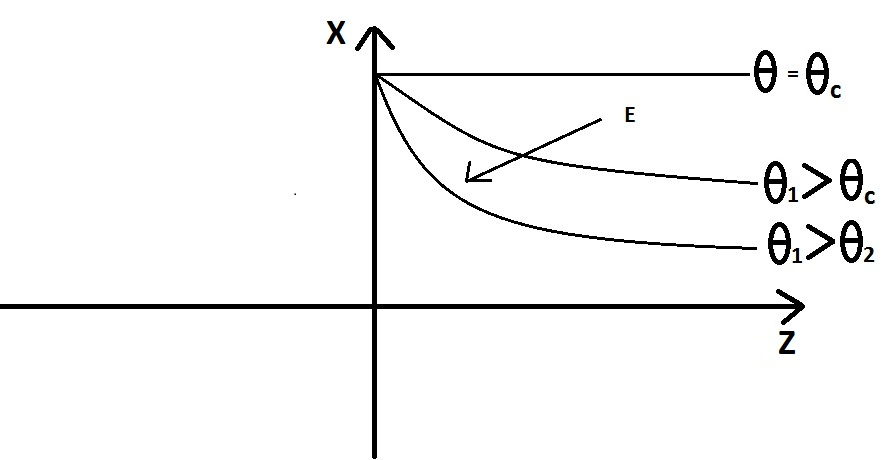
\includegraphics[width=.7\linewidth]{\pathtopartone/graphics/fig322}
\caption{Graph of travelling waves fields}
\end{figure}

At angle $\theta_t >$ $\theta_c$ the decay is faster as shown in the graphs. 
So as the angle of incidence increases more and more beyond the critical angle, the field gets more and more confined towards the dielectric interface. So at the critical angle, the field thermally extends up to infinity at a constant amplitude. The important observation is the field never goes to zero in medium 2 under no condition. The field is always non-zero in medium 2. Theoretically, no matter how small this amplitude is, it will extend up to infinity in the direction Z, it gets closer and closer to zero but never zero.
So when total internal reflection takes place from medium 1 at the high school level, it was like the total power reflected medium 1 and nothing existed in medium 2. There was no discussion at all as to what was the behaviour of the fields in 2 or the role medium 2 needed to play in total internal reflection. Once we had the critical condition for total internal reflection satisfied, we didn't bother about the point beyond the boundary into medium 2. Now we can't ignore the region in medium 2 beyond the boundary. The fields have to exist in the form shown in medium 2 for total internal reflection to take place, and they are as important as the fields in medium 1. The field in medium 2 is required for us to satisfy the continuity equation at the boundary. It is these fields in medium 2 that is supporting the total internal reflection phenomenon. If any disturbance is created to these fields in the medium from fig 32.2, the total internal reflection phenomenon is also disturbed and we cannot have total internal reflection, also the power will flow to medium 2. So to have a good total internal reflection phenomenon, we must have the field in medium 2 as confined to the interface as much as possible. That means we must launch a wave with an angle larger than the critical angle for as much as possible so that the field will die down in medium 2 as fast as possible and so that it is confined to a thickness Z in medium 2 that is extremely small.

Secondly, we must provide a certain region from the dielectric interface in medium 2 of thickness Z(ideally Z should be at infinity) where the fields in medium 2 are protected. If these two conditions are guaranteed, we have a total internal reflection phenomenon in the medium. Theoretically, unless we provide an infinite medium in 2, and the fields properly protected in medium 2, we cannot have a total internal reflection phenomenon.

\section{Reactive Fields}

We conclude that when total internal reflection takes place, the field in medium 2 exists, and the transmission coefficient is not zero. When the total power is reflected, $|\Gamma| = 1$. It doesn't mean that the transmission coefficient is zero. The transmission coefficient doesn't mean that there is a power flow in medium 2. As we have seen the fields which are dying down in medium 2 are the ones which do not constitute power flow as the wave is not travelling inside the medium. The wave is still travelling in the x direction along the dielectric interface. There is no power flow in the Z direction, but the fields exist. So we should clearly understand the difference between having fields and no power flow and having fields with power flow. You may have electric and magnetic fields and they may constitute power flow, as we have seen in earlier cases.

However, we might have a situation like this where we have electric and magnetic fields but there is no power flow. In the electrical circuit terminology, we can call this field REACTIVE FIELDS, they have the energy stored in the transient phase when the field is being set up but no power flow. We visualize it as when the wave is incident on the interface or boundary when the wave is being set up, there is some power flow into the second medium. That power flow gets stored in the energy in the second medium in the fields. These fields are decaying fields. Once these fields are set up, up in the steady state, no net power flows in the second medium and the power flow is essential in medium 1. These fields in medium 2 are referred to as EVENESCENT FILEDS (reactive fields). They will exist in medium 2 without constituting any power flow. The power flow will exist in the interface in the direction of x. Now for medium 1, we had a wave incident on it and another one which is reflected from the interface into medium 1. There is arbitrary phase change at the point of incidence and reflection as shown below.
\begin{figure}[h]
\centering
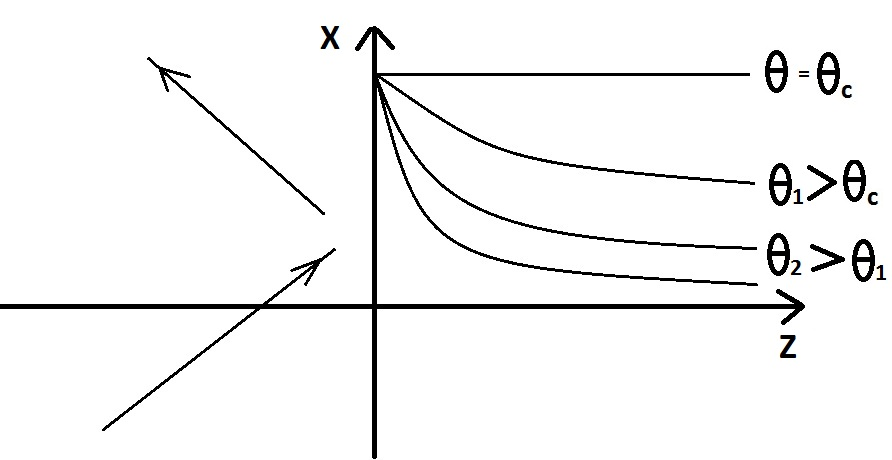
\includegraphics[width=.7\linewidth]{\pathtopartone/graphics/fig323}
\caption{Graph of incidence and reflection}
\end{figure}

Fields in medium 1
\begin{equation}
E_i = E_i e^{- \jmath \beta_1(x\sin\theta_i + z\cos\theta_i)}
\end{equation}
\begin{equation}
E_r = E_r e^{- \jmath \beta_1(x\sin\theta_i - z\cos\theta_i)}
\end{equation}
\begin{equation*}
E = E_i + E_r
\end{equation*}
\begin{equation*}
E = E_i e^{- \jmath \beta_1x\sin\theta_i}\{ 1e^{- \jmath \beta_1z\cos\theta_i} + e^{\jmath \theta}
e^{\jmath \beta_1\cos\theta_i} \}
\end{equation*}
Depending on the phase change $\theta_1$ at $z = 0$ the amplitude can be changed. M and N waves will create constructive or destructive interference as we saw in the case of transmission lines. 

So in medium 1 from the equation, we have a fully developed standing wave in z directions but a travelling wave in x direction. In medium 2 it was an exponentially decaying field and a travelling wave in the x direction with the same phase constant as in medium 1 travelling wave in the x direction. We plot the fields now in the two media we have depending upon the phase of reflection $\phi$, so the field distribution is like a corrugated surface in medium 1 and a decaying field in medium 2. The constant phase plane is determined by $e^{- \jmath \beta_1x\sin\theta_i}$. So the constant phase plane is the yz plane. The constant amplitude plane is in the XY plane. So this complex amplitude distribution of the wave travels in the x direction with a phase constant $\beta_1\sin\theta_i$.
\begin{figure}[h]
\centering
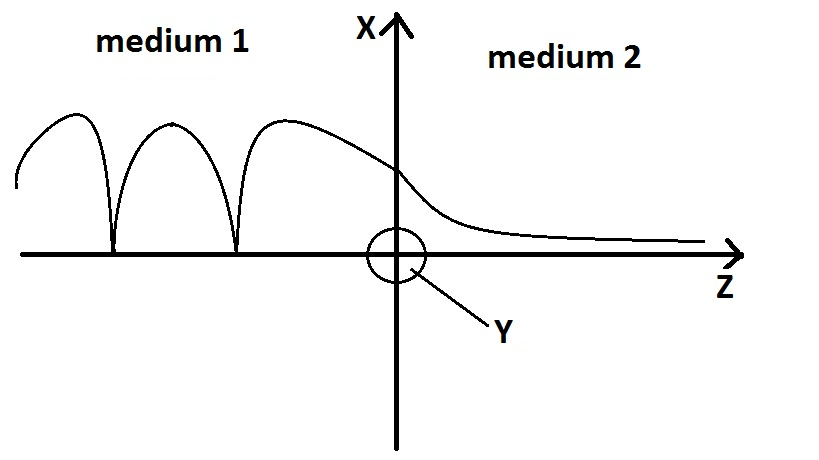
\includegraphics[width=.7\linewidth]{\pathtopartone/graphics/fig324}
\caption{Graph of field distribution}
\end{figure}

So whenever total internal reflection occurs, you have this complex distribution of amplitude in space, one side exponentially decaying fields, the other side standing wave kind of fields. This amplitude distribution travels in the x direction with a phase velocity $\beta_1\sin\theta_i$. So the phase velocity in the x direction $V_px = \frac{\omega}{\beta_1\sin\theta_i}$. What is the direction of net power flow? The field in medium 2 does not constitute any wave, so no power flow in the Z direction. With no power flow in the z direction in medium 2, there can be no power flow in the z direction in medium 1 also. Since if the power had come from medium 1 in the z direction, and the power can't flow in medium 2, the interface does not consume power since we are talking of a completely lossless medium. Hence whatever power came from the medium 1 incident on the boundary, essentially gets reflected to give us the power flow perpendicular to the interface. Along the interface, there is a power flow, we had phase velocity. So when the total internal reflection phenomenon takes place, the net power flow is along the interface. Or in another word, the dielectric interface is capable of guiding electromagnetic energy.

\section{Wave Guides}

So we can make use of a dielectric interface for guiding electromagnetic energy along the line. Precisely this is what is used in structures called WAVEGUIDES, and especially when we talk about dielectric media this is what happens in optical fibres. An optical fibre is nothing but a structure having a dielectric interface. So with a wave launched at an angle $\theta_i > \theta_c$,
then there is a total internal reflection in medium 1. The field in medium 2 will exponentially decay along the x direction. Power flow will be in the z direction based on the coordinate axes used for this illustration.

So if we create some structure like this, it can carry electromagnetic energy over a long distance without any loss as such. Energy is confined in the region of $n_1$ and it will propagate along z direction as a result of total internal reflection. So total internal reflection has played important role in modern optical communication and helped in the design of structures called optic fibres. 
